
%%%%%%%%%%%%%%%%%%%%%%%%%%%%%%%%%%%%%%%%%%%%%%%%%%

\documentclass{beamer}
% \usepackage{graphicx}
\usepackage{beamerthemesplit}
\usepackage{color}

% \usepackage{color}
% \input{preamble1.tex}

% End of package list and other added codes.

%%%%%%%%%%%%%%%%%%%%%%%%%%%%%%%%%%%%%%%%%%%%%%%%%%

% \titlegraphic{\includegraphics[width=\textwidth,height=.5\textheight]{someimage}}
% \titlegraphic{\includegraphics[scale =  0.05 ]{C1_Core_2CG_RGB.jpg}}

\title[Forecast Intervals for the
    Area Under the ROC Curve]{Forecast Intervals for the \\
    Area Under the ROC Curve \\
    with a Time-varying Population}



\author[Lealand Morin, University of Central Florida]{Lealand Morin}

\institute[University of Central Florida]
{
    Department of Economics \\
    College of Business Administration \\
    University of Central Florida
    % Capital One
    % \includegraphics[scale =  0.05 ]{C1_Core_2CG_RGB.jpg}
}

% \logo{\includegraphics[scale =  0.025 ]{C1_Core_2CG_RGB.jpg}}

%\author{Lee Morin}
%\institute[Queen's University]
%{
%    Department of Economics \\
%    Queen's University
%}

% \date{\today}
\date{October 19, 2018}


%%%%%%%%%%%%%%%%%%%%%%%%%%%%%%%%%%%%%%%%%%%%%%%%%%


\begin{document}


%%%%%%%%%%%%%%%%%%%%%%%%%%%%%%%%%%%%%%%%%%%%%%%%%%

\frame{\titlepage}
% \frametitle{Agenda}

\section[Outline]{}

\frame{\tableofcontents}


%%%%%%%%%%%%%%%%%%%%%%%%%%%%%%%%%%%%%%%%%%%%%%%%%%


\section{Introduction}


%%%%%%%%%%%%%%%%%%%%%%%%%%%%%%%%%%%%%%%%%%%%%%%%%%

\begin{frame}
\frametitle{Predicting Performance of Classification Models}

% Tagline goes here
\begin{itemize}
    \item \textbf{What:} Method for calculating a forecast interval for the Area Under the ROC curve (AUROC)
    \begin{itemize}
        \item Area under the Receiver Operating Characteristic (ROC) curve: \\
        quality of a signal for predicting an outcome
        % is a measure of quality of a signal for predicting an outcome
        % \item In predictive modeling, it is often used as a measure of performance of a classification model
        \item Predictive modeling: performance of a classification model
    \end{itemize}
    \item \textbf{Why:} Characterize the likely range of model performance while a model is used for prediction
    \begin{itemize}
        \item In practice, businesses will use model until:
        \begin{itemize}
            \item Performance (AUROC) degrades
            \item Population changes
        \end{itemize}
    \end{itemize}
    \item \textbf{How:} Measure the variation in AUROC in terms of the variation in the underlying distribution of predictive variables
    \begin{itemize}
        \item Not only from sampling variation from a fixed distribution
    \end{itemize}
\end{itemize}

\end{frame}


%%%%%%%%%%%%%%%%%%%%%%%%%%%%%%%%%%%%%%%%%%%%%%%%%%

\begin{frame}
\frametitle{Measuring Predictive Value of Classification Models}

Receiver Operating Characteristic Curve: \\
True Positive Rate vs. False Positive Rate
\begin{figure}
    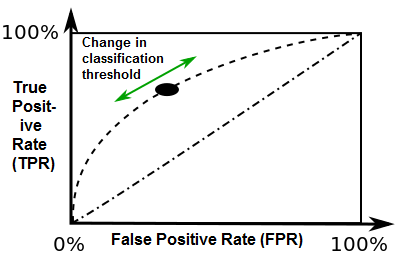
\includegraphics[scale =  0.75 ]{Figs/ROC_curve_3.png}
\end{figure}

\end{frame}


%%%%%%%%%%%%%%%%%%%%%%%%%%%%%%%%%%%%%%%%%%%%%%%%%%

\begin{frame}
\frametitle{Measuring Predictive Value of Classification Models}

Definition of AUROC
\begin{itemize}
    \item Direct definition: Calculation of area by integration
    \begin{itemize}
        \item $\int_{-\infty}^{\infty} TPR(t) [-FPR^{\prime}(t)] dt $
    \end{itemize}
    \item Direct definition: Pairwise comparison of correct ordering of predictions for all pairs of predictions % from positive and negative outcomes
    \begin{itemize}
        \item $\hat{A} = \hat{\Pr} \{ y > x \} = \frac{1}{m n} \sum_{i = 1}^{m} \sum_{j = 1}^{n} I_{\left\{ y_j > x_i \right\}}$
    \end{itemize}
    \item In words: If you were to pick a pair of predictions, drawn randomly from predictions corresponding to pairs of the positive ($y$) and negative ($x$) outcomes, the AUROC is the probability that these predictions are correctly ordered.
\end{itemize}

\end{frame}


%%%%%%%%%%%%%%%%%%%%%%%%%%%%%%%%%%%%%%%%%%%%%%%%%%

\begin{frame}
\frametitle{Graphical Interpretation of AUROC}

Volume Under the Joint distribution of Predictor Variables
\begin{figure}
    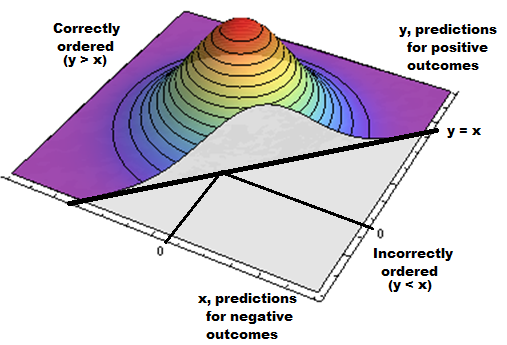
\includegraphics[scale =  0.65 ]{Figs/AUROC_vol_3.png}
\end{figure}

\end{frame}


%%%%%%%%%%%%%%%%%%%%%%%%%%%%%%%%%%%%%%%%%%%%%%%%%%

\begin{frame}
\frametitle{An Important Correspondence for Classification Models}

%Predictive value of variables
%(relation of score to positives and negatives)
%
%Difference in distributions of variables
%(positives vs. negatives)
Predicting Outcomes vs. Measuring Difference

\begin{figure}
        \begin{minipage}[b]{0.45\linewidth}
            \centering
            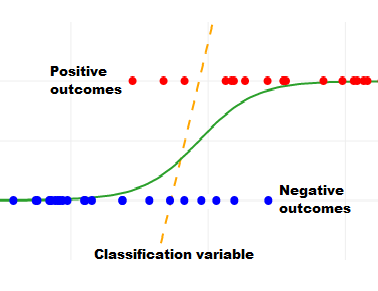
\includegraphics[width=\textwidth]{Figs/LogisticReg_5.png}
            % \caption{Predictive value of variables \\ (relation of score to positives and negatives)}
            \caption{Predictive value of classification variables}
        \end{minipage}
        \hspace{0.5cm}
        \begin{minipage}[b]{0.45\linewidth}
            \centering
            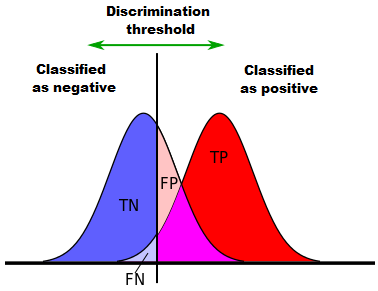
\includegraphics[width=\textwidth]{Figs/ROC_distns_1.png}
            % \caption{Difference in distributions of variables \\ (positives vs. negatives)}
            \caption{Difference in the distributions of variables}
        \end{minipage}
    % 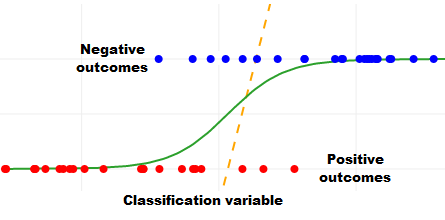
\includegraphics[scale =  0.5 ]{Figs/LogisticReg_3.png}%
    % 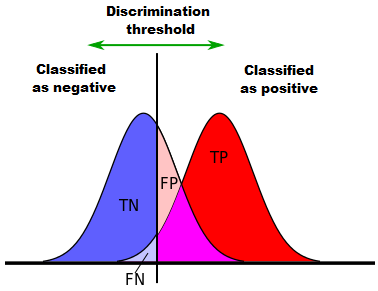
\includegraphics[scale =  0.5 ]{Figs/ROC_distns_1.png}
\end{figure}

\end{frame}


%%%%%%%%%%%%%%%%%%%%%%%%%%%%%%%%%%%%%%%%%%%%%%%%%%

\begin{frame}
\frametitle{Predicting Performance of Classification Models}

% Conclusion: Variation of distributions of scores is of paramount importance
Conclusion: Variation of distributions is of paramount importance
\begin{itemize}
    \item AUROC statistic is closely related to the pairs of distributions
     \item In practice, track performance of model while in use
     \begin{itemize}
         \item take AUROC measurements periodically
     % \end{itemize}
    % \item In practice, business users would track evolution of distributions of predictions
    % \begin{itemize}
        \item take periodic measurements of changes in distributions to measure deviations from build sample
    \end{itemize}
    \item Extreme changes in either would trigger rebuild of the model
    \item Forecast intervals should allow for this level of variability
\end{itemize}

\end{frame}


%%%%%%%%%%%%%%%%%%%%%%%%%%%%%%%%%%%%%%%%%%%%%%%%%%


\section{Contribution}


%%%%%%%%%%%%%%%%%%%%%%%%%%%%%%%%%%%%%%%%%%%%%%%%%%

\begin{frame}
\frametitle{Predicting Performance of Classification Models}

% Contribution:
Calculation of forecast intervals:
% \begin{itemize}
    % \item Existing literature seeks to characterize variability due to \emph{sampling variation}
    % \item In this paper, I allow for additional variation in the sample due to changes in the underlying distribution
    % \item How far would the AUROC move before model rebuild is triggered?
    % \item Method of calculation:
    \begin{itemize}
        \item[1] Build model from entire sample and measure AUROC
        \item[2] Measure distance between distributions
            \begin{itemize}
                \item by dividing sample into a series of subsamples
                \item by specifying a model for the evolution of the distributions
            \end{itemize}
        \item[3] Calculate extreme AUROC values that correspond to movements a specified distance away from the full sample
    \end{itemize}
% \end{itemize}

\end{frame}


%%%%%%%%%%%%%%%%%%%%%%%%%%%%%%%%%%%%%%%%%%%%%%%%%%


\subsection{Optimization Problem}


%%%%%%%%%%%%%%%%%%%%%%%%%%%%%%%%%%%%%%%%%%%%%%%%%%

\begin{frame}
\frametitle{Optimization Problem}

% To find the upper bound of the prediction interval, $A^{(U)}$, this optimization problem is

Find the highest value of the AUROC, $A^{(U)}$, a specified distance from observed distribution \\
$\max_{\mathbf{u}, \mathbf{v}} \frac{1}{m n} \sum_{i = 1}^{m} \sum_{j = 1}^{n} u_i v_j I_{\left\{ y_j > x_i \right\}}$
\begin{itemize}
    % \item $\min_{\mathbf{u},\mathbf{v}}
    %     D(\mathbf{u},\mathbf{f}, \mathbf{v},\mathbf{g})$
    \item subject to
    $D(\mathbf{u} \otimes \mathbf{v}, \mathbf{f} \otimes \mathbf{g}) = \bar{D}$,
    \item unit mass constraints
    $\sum_{i = 1}^{m} u_i = 1, \quad \sum_{j = 1}^{n} v_j = 1$,
    \item nonnegativity constraints
    $ \left\{ u_i  \geq 0 \right\}_{i=1}^{m}, \quad \left\{ v_j \geq 0 \right\}_{j=1}^{n}$
    \item where $\mathbf{f}$ and $\mathbf{g}$ are the observed distributions of classification variables for positive and negative cases, respectively,
    while $\mathbf{u}$ and $\mathbf{v}$ are the weights with distance $\bar{D}$
\end{itemize}

\end{frame}

%%%%%%%%%%%%%%%%%%%%%%%%%%%%%%%%%%%%%%%%%%%%%%%%%%%

\begin{frame}
\frametitle{Dual Problem}

Find \emph{minimum} distance from observed distribution and a distribution with a particular AUROC \\
$\min_{\mathbf{u}, \mathbf{v}}
        KLD(\mathbf{u} \otimes \mathbf{v}, \mathbf{f} \otimes \mathbf{g})$
\begin{itemize}
    % \item $\min_{\mathbf{u},\mathbf{v}}
    %     D(\mathbf{u},\mathbf{f}, \mathbf{v},\mathbf{g})$
    \item subject to
    $\frac{1}{m n} \sum_{i = 1}^{m} \sum_{j = 1}^{n} u_i v_j I_{\left\{ y_j > x_i \right\}} = A_0$,
    \item unit mass constraints
    $\sum_{i = 1}^{m} u_i = 1, \quad \sum_{j = 1}^{n} v_j = 1$,
    \item nonnegativity constraints
    $ \left\{ u_i  \geq 0 \right\}_{i=1}^{m}, \quad \left\{ v_j \geq 0 \right\}_{j=1}^{n}$
    \item where $\mathbf{f}$ and $\mathbf{g}$ are the observed distributions of classification variables for positive and negative cases, respectively,
    while $\mathbf{u}$ and $\mathbf{v}$ are the closest weights that satisfy $A = A_0$
\end{itemize}

\end{frame}

%%%%%%%%%%%%%%%%%%%%%%%%%%%%%%%%%%%%%%%%%%%%%%%%%%%

\begin{frame}
\frametitle{Optimum}

Fixed points from first order conditions
\begin{itemize}
    \item $\frac{d D(\mathbf{u},\mathbf{f})}{d u_i} = \lambda \sum_{j = 1}^{n} v_j I_{\left\{ y_j > x_i \right\}} + \gamma_x + \delta_{x,i},
    i = 1, \dots, m$
    \item $\frac{d D(\mathbf{v},\mathbf{g})}{d v_j} = \lambda \sum_{i = 1}^{m} u_i I_{\left\{ y_j > x_i \right\}} + \gamma_y + \delta_{y,i},
    j = 1, \dots, n$
    \item Solved with the recurrence relations (for a particular distance function)
    \begin{itemize}
        % \item $u_i = \exp{ \left\{ 1 + \ln f_i + u_i \ln f_i
        %         + \lambda \sum_{j = 1}^{n} v_j I_{\left\{ y_j > x_i \right\}} + \gamma_x \right\} }$
        \item $u_i^{(t+1)} = k_x f_i ^{1 + u_i^{(t)}}
                \exp{ \left\{ \lambda \sum_{j = 1}^{n} v_j^{(t)} I_{\left\{ y_j > x_i \right\}} \right\} }$
        % \item $v_j = \exp{ \left\{ 1 + \ln g_j + v_j \ln g_j
        %         + \lambda \sum_{i = 1}^{m} u_i I_{\left\{ y_j > x_i \right\}} + \gamma_y \right\} }$
        \item $v_j^{(t+1)} = k_y g_j ^{1 + v_j^{(t)}}
                \exp{ \left\{ \lambda \sum_{i = 1}^{m} u_i^{(t)} I_{\left\{ y_j > x_i \right\}}  \right\} }$
    \end{itemize}
    \item $k_x$ and $k_y$ are normalizing constants and Lagrange multiplier $\lambda$ is the step size.
\end{itemize}

\end{frame}

%%%%%%%%%%%%%%%%%%%%%%%%%%%%%%%%%%%%%%%%%%%%%%%%%%%


\subsection{Comparison}


%%%%%%%%%%%%%%%%%%%%%%%%%%%%%%%%%%%%%%%%%%%%%%%%%%

\begin{frame}
\frametitle{Competing Procedures}

% Confidence Intervals in Literature
\begin{itemize}

    \item Parametric models:
    \begin{itemize}
        \item Binormal model: $[\Phi(\tilde{z}_{\alpha/2}), \Phi(\tilde{z}_{1-\alpha/2})]$
        \item Biexponential model: $[\hat{A} \pm  z_{1-\alpha/2} \hat{\sigma}_A]$, with \\
        $\sigma^2_A = \frac{1}{mn} \{ A(1 - A) + (n - 1)(P_{yyx} - A^2) + (m - 1)(P_{yxx} - A^2) \}$,
        $P_{yyx} = A/(2-A)$, $P_{yxx} = 2A^2/(1+A)$
    \end{itemize}

    \item Empirical distribution (DeLong et. al.): \\
    $P_{yyx} = \frac{1}{mnn} \sum_i \sum_j \sum_k I_{\left\{ y_j > x_i \cap y_k > x_i \right\}}$ \\
    % $\qquad\qquad\qquad\qquad$ and
    $P_{yxx} = \frac{1}{mmn} \sum_i \sum_j \sum_k I_{\left\{ y_j > x_i \cap y_j > x_k \right\}}$

    \item Bootstrap: $[\hat{A}_{\alpha/2}^*, \hat{A}_{1-\alpha/2}^*]$

    \item Upper bound of variance: $\sigma^2_{max} = \frac{A(1-A)}{\min\{ m, n \}} \big( \leq \frac{1}{4 \min\{ m, n \} } \big) $

    \item Fixed error rate: Interval depends on a specified error rate.

\end{itemize}

\end{frame}

%%%%%%%%%%%%%%%%%%%%%%%%%%%%%%%%%%%%%%%%%%%%%%%%%%%

\begin{frame}
\frametitle{Prediction Intervals Expanding with Distance}

% Expanding Prediction Intervals with Distance
\vspace*{-0.25cm}
\begin{figure}
    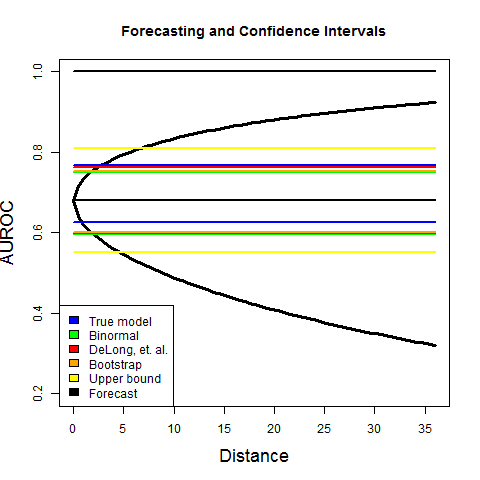
\includegraphics[scale =  0.4 ]{Figs/Forecast_int_1.png}
\end{figure}

\end{frame}


%%%%%%%%%%%%%%%%%%%%%%%%%%%%%%%%%%%%%%%%%%%%%%%%%%


% \section{Results}
\subsection{Simulations}


%%%%%%%%%%%%%%%%%%%%%%%%%%%%%%%%%%%%%%%%%%%%%%%%%%

\begin{frame}
\frametitle{Predicting Performance of Classification Models}

Structure of Simulation
\begin{itemize}
    \item Regime-switching model
    \begin{itemize}
        \item 2 states, high- and low-AUROC regimes, equally probable
        \item past regimes known, future unknown
    \end{itemize}
    \item Measure AUROC from both regimes
    \item Measure distance between distributions in regimes and full sample
    \item Calculate extreme AUROC values that correspond to movements away from full sample, using distances between distributions
\end{itemize}

\end{frame}


%%%%%%%%%%%%%%%%%%%%%%%%%%%%%%%%%%%%%%%%%%%%%%%%%%

\begin{frame}
\frametitle{Simulation Results}

%Tables for first case
%\begin{figure}
%    
\includegraphics[scale =  0.75 ]{Figs/ThisIsNotSkyNetLogo.png}
%\end{figure}


%%%%%%%%%%%%%%%%%%%%%%%%%%%%%%%%%%%%%%%%%%%%%%%%%%%%%%%%%%%%%%%%%%%%%%%%%%%%%%%%%%%%%%%%%%%%%%%%%%%%%%%%%%%%%%%

Coverage Rates \\
True values: $A_L = 0.68, A_H = 0.72$

\begin{figure}[h!]

\begin{center}

    % \hline
    % \caption{Rates of Coverage and Correct Forecasts ($A_L = 0.68, A_H = 0.72$)} \label{fig:Coverage1}

    % \hline
    \begin{tabular}{l c c }

    Method & Coverage Rate & Correct Forecast Rate \\

    \hline

    %[1] "Coverage rates for n = 1100, A_L = 0.680000, A_H = 0.720000"
%               method coverage  forecast
%    1:      Bi-normal   0.8265 0.6612295
%    2: DeLong et. al.   0.8395 0.6689495
%    3:      Bootstrap   0.8310 0.6616050
%    4:    Upper Bound   0.9885 0.9074855
%    5:       Forecast   0.9955 0.9600615


          Bi-normal &  0.8265 & 0.6612 \\
     DeLong et. al. &  0.8395 & 0.6689 \\
          Bootstrap &  0.8310 & 0.6616 \\
        Upper Bound &  0.9885 & 0.9074 \\
           Forecast &  0.9955 & 0.9600 \\


    \hline

    \end{tabular}

    % \hline

\end{center}

%    \footnotesize
%
%        \textbf{Rates of Coverage and Correct Forecasts:}
%        Coverage rates are the proportion of confidence intervals that contain the true values of the AUROC.
%        Correct forecast rates are the proportion of confidence intervals that contain the estimated values of the AUROC.
%        Number of replications is $1,000$ for all models, with $399$ bootstrap replications for bootstrap confidence intervals.
%        Data generating process is a two-state regime-switching model with a bi-normal classification model in each state,
%        with true AUROC values of $0.68$ in the low state and $0.72$ in the high state.
%        % Bi-normal models have standard deviations of $1/sqrt{2}$.
%        % Positive distributions have


    % \hline



\end{figure}


%%%%%%%%%%%%%%%%%%%%%%%%%%%%%%%%%%%%%%%%%%%%%%%%%%%%%%%%%%%%%%%%%%%%%%%%%%%%%%%%%%%%%%%%%%%%%%%%%%%%%%%%%%%%%%%



\end{frame}


%%%%%%%%%%%%%%%%%%%%%%%%%%%%%%%%%%%%%%%%%%%%%%%%%%

\begin{frame}
\frametitle{Simulation Results}

%Plot confidence intervals for an example
%\begin{figure}
%    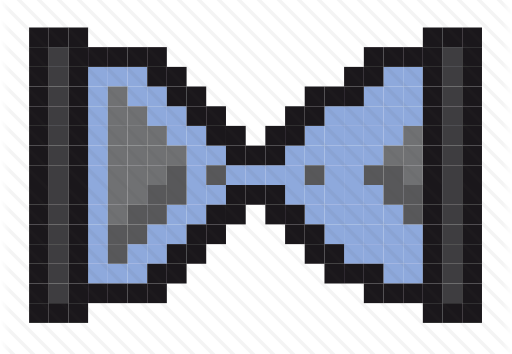
\includegraphics[scale =  0.5 ]{Figs/hourglass_icon_2.png}
%\end{figure}


%%%%%%%%%%%%%%%%%%%%%%%%%%%%%%%%%%%%%%%%%%%%%%%%%%%%%%%%%%%%%%%%%%%%%%%%%%%%%%%%%%%%%%%%%%%%%%%%%%%%%%%%%%%%%%%


\begin{figure}[h!]

\begin{center}

    % \hline
    \caption{Rates of Coverage and Correct Forecasts ($A_L = 0.65, A_H = 0.75$)} \label{fig:Coverage1}

    % \hline
    \begin{tabular}{l c c }

    Method & Coverage Rate & Correct Forecast Rate \\

    \hline
    
%    [1] "Coverage rates for n = 1100, A_L = 0.650000, A_H = 0.750000"
%           method coverage  forecast
%    1:      Bi-normal   0.2360 0.3427380
%    2: DeLong et. al.   0.2470 0.3515930
%    3:      Bootstrap   0.2455 0.3453490
%    4:    Upper Bound   0.7725 0.6615905
%    5:       Forecast   0.9795 0.9259675


          Bi-normal &  0.2360 & 0.3427 \\
     DeLong et. al. &  0.2470 & 0.3515 \\
          Bootstrap &  0.2455 & 0.3453 \\
        Upper Bound &  0.7725 & 0.6615 \\
           Forecast &  0.9795 & 0.9259 \\


    \hline

    \end{tabular}

    % \hline

\end{center}

    \footnotesize

        \textbf{Rates of Coverage and Correct Forecasts:}
        Coverage rates are the proportion of confidence intervals that contain the true values of the AUROC.
        Correct forecast rates are the proportion of confidence intervals that contain the estimated values of the AUROC.
        Number of replications is $1,000$ for all models, with $399$ bootstrap replications for bootstrap confidence intervals.
        Data generating process is a two-state regime-switching model with a bi-normal classification model in each state,
        with true AUROC values of $0.65$ in the low state and $0.75$ in the high state.
        % Bi-normal models have standard deviations of $1/sqrt{2}$.
        % Positive distributions have


    % \hline



\end{figure}


%%%%%%%%%%%%%%%%%%%%%%%%%%%%%%%%%%%%%%%%%%%%%%%%%%%%%%%%%%%%%%%%%%%%%%%%%%%%%%%%%%%%%%%%%%%%%%%%%%%%%%%%%%%%%%%



\end{frame}


%%%%%%%%%%%%%%%%%%%%%%%%%%%%%%%%%%%%%%%%%%%%%%%%%%

\begin{frame}
\frametitle{Simulation Results}

%Tables for remaining cases
%\begin{figure}
%    
\includegraphics[scale =  0.75 ]{Figs/ThisIsNotSkyNetLogo.png}
%\end{figure}


%%%%%%%%%%%%%%%%%%%%%%%%%%%%%%%%%%%%%%%%%%%%%%%%%%%%%%%%%%%%%%%%%%%%%%%%%%%%%%%%%%%%%%%%%%%%%%%%%%%%%%%%%%%%%%%


\begin{figure}[h!]

\begin{center}

    % \hline
    \caption{Rates of Coverage and Correct Forecasts ($A_L = 0.75, A_H = 0.80$)} \label{fig:Coverage1}

    % \hline
    \begin{tabular}{l c c }

    Method & Coverage Rate & Correct Forecast Rate \\

    \hline
    
%    [1] "Coverage rates for n = 1100, A_L = 0.750000, A_H = 0.800000"
%           method coverage  forecast
%    1:      Bi-normal   0.6805 0.5912520
%    2: DeLong et. al.   0.6845 0.5979860
%    3:      Bootstrap   0.6730 0.5889715
%    4:    Upper Bound   0.9665 0.8654290
%    5:       Forecast   0.9940 0.9451650
    
    
          Bi-normal &  0.6805 & 0.5912 \\
     DeLong et. al. &  0.6845 & 0.5979 \\
          Bootstrap &  0.6730 & 0.5889 \\
        Upper Bound &  0.9665 & 0.8654 \\
           Forecast &  0.9940 & 0.9451 \\

    \hline

    \end{tabular}

    % \hline

\end{center}

    \footnotesize

        \textbf{Rates of Coverage and Correct Forecasts:}
        Coverage rates are the proportion of confidence intervals that contain the true values of the AUROC.
        Correct forecast rates are the proportion of confidence intervals that contain the estimated values of the AUROC.
        Number of replications is $1,000$ for all models, with $399$ bootstrap replications for bootstrap confidence intervals.
        Data generating process is a two-state regime-switching model with a bi-normal classification model in each state,
        with true AUROC values of $0.75$ in the low state and $0.80$ in the high state.
        % Bi-normal models have standard deviations of $1/sqrt{2}$.
        % Positive distributions have


    % \hline



\end{figure}


%%%%%%%%%%%%%%%%%%%%%%%%%%%%%%%%%%%%%%%%%%%%%%%%%%%%%%%%%%%%%%%%%%%%%%%%%%%%%%%%%%%%%%%%%%%%%%%%%%%%%%%%%%%%%%%



\end{frame}


%%%%%%%%%%%%%%%%%%%%%%%%%%%%%%%%%%%%%%%%%%%%%%%%%%

\begin{frame}
\frametitle{Simulation Results}

%Tables for remaining cases
%\begin{figure}
%    
\includegraphics[scale =  0.75 ]{Figs/ThisIsNotSkyNetLogo.png}
%\end{figure}


%%%%%%%%%%%%%%%%%%%%%%%%%%%%%%%%%%%%%%%%%%%%%%%%%%%%%%%%%%%%%%%%%%%%%%%%%%%%%%%%%%%%%%%%%%%%%%%%%%%%%%%%%%%%%%%


\begin{figure}[h!]

\begin{center}

    % \hline
    \caption{Rates of Coverage and Correct Forecasts ($A_L = A_H = 0.70$)} \label{fig:Coverage1}

    % \hline
    \begin{tabular}{l c c }

    Method & Coverage Rate & Correct Forecast Rate \\

    \hline
    
%    [1] "Coverage rates for n = 1100, A_L = 0.700000, A_H = 0.700000"
%           method coverage  forecast
%    1:      Bi-normal    0.951 0.7402125
%    2: DeLong et. al.    0.944 0.7477020
%    3:      Bootstrap    0.941 0.7386815
%    4:    Upper Bound    1.000 0.9464325
%    5:       Forecast    0.999 0.9702450
    
    
          Bi-normal  &  0.951 & 0.7402 \\
     DeLong et. al.  &  0.944 & 0.7477 \\
          Bootstrap  &  0.941 & 0.7386 \\
        Upper Bound  &  1.000 & 0.9464 \\
           Forecast  &  0.999 & 0.9702 \\

    \hline

    \end{tabular}

    % \hline

\end{center}

    \footnotesize

        \textbf{Rates of Coverage and Correct Forecasts:}
        Coverage rates are the proportion of confidence intervals that contain the true values of the AUROC.
        Correct forecast rates are the proportion of confidence intervals that contain the estimated values of the AUROC.
        Number of replications is $1,000$ for all models, with $399$ bootstrap replications for bootstrap confidence intervals.
        Data generating process is a two-state regime-switching model with a bi-normal classification model in each state,
        with true AUROC values of $0.70$ in both states.
        % Bi-normal models have standard deviations of $1/sqrt{2}$.
        % Positive distributions have


    % \hline



\end{figure}


%%%%%%%%%%%%%%%%%%%%%%%%%%%%%%%%%%%%%%%%%%%%%%%%%%%%%%%%%%%%%%%%%%%%%%%%%%%%%%%%%%%%%%%%%%%%%%%%%%%%%%%%%%%%%%%



\end{frame}


%%%%%%%%%%%%%%%%%%%%%%%%%%%%%%%%%%%%%%%%%%%%%%%%%%


\section{Methods}
\subsection{Measuring Distance}


%%%%%%%%%%%%%%%%%%%%%%%%%%%%%%%%%%%%%%%%%%%%%%%%%%

\begin{frame}
\frametitle{A ``Non-parametric'' Solution}


\begin{itemize}
    \item AUROC is inherently nonparametric measure of performance
    \begin{itemize}
        \item General distaste for parametric assumptions, particularly when not supported by the data
        \item Little justification to impose parametric specification for variation in distributions, when parametric distributions are not used for the distributions themselves
        \item Still, parametric specification would work
    \end{itemize}
    \item Change in distribution is summarized by a distance measurement
    \begin{itemize}
        \item Forecast interval is a function of the distance measurement
    \end{itemize}
\end{itemize}

\end{frame}

%%%%%%%%%%%%%%%%%%%%%%%%%%%%%%%%%%%%%%%%%%%%%%%%%%%

\begin{frame}
\frametitle{Distance Function}

Kullback-Leibler Divergence Criterion
\begin{itemize}
\item A criterion for discriminating between distributions
    \item Definition
    \begin{itemize}
        \item $KLD(f_1, f_2) = \sum_{k = 1}^{K} \left\{ \bigg( f_1(t_k) - f_2(t_k) \bigg)
        \log \left( \frac{f_1(t_k)}{f_2(t_k)} \right) \right\}$
        \item where $f_1$ and $f_2$ are two density functions
    \end{itemize}
\end{itemize}

\end{frame}

%%%%%%%%%%%%%%%%%%%%%%%%%%%%%%%%%%%%%%%%%%%%%%%%%%%

\begin{frame}
\frametitle{Kullback-Leibler Divergence}

Difference and Log-difference for Two Normal Densities
\vspace*{-0.25cm}
\begin{figure}
    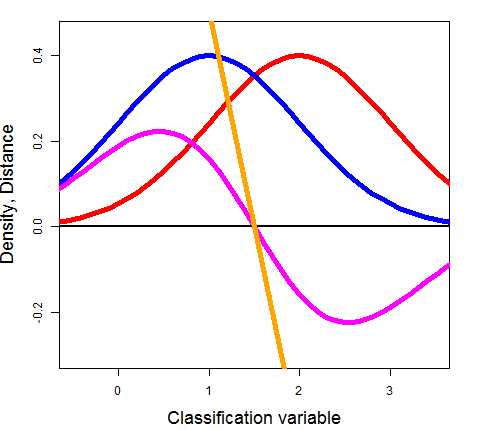
\includegraphics[scale =  0.40 ]{Figs/KLD_calc_3.png}
\end{figure}
\vspace*{-0.25cm}
Terms in $KLD(\textcolor{blue}{f_1}, \textcolor{red}{f_2})
 = \sum_{k = 1}^{K} \left\{ \textcolor{magenta}{\big( f_1(t_k) - f_2(t_k) \big)}
        \textcolor{orange}{\log \left( \frac{f_1(t_k)}{f_2(t_k)} \right)} \right\}$
\end{frame}


%%%%%%%%%%%%%%%%%%%%%%%%%%%%%%%%%%%%%%%%%%%%%%%%%%

\begin{frame}
\frametitle{Distance Function}

Why Kullback-Leibler Divergence?
\begin{itemize}
    \item More weight on tails: Penalty for deviations in low density has more influence on variation of AUROC, since the variation in AUROC is generated where the densities overlap
    \item Information-theoretic justification: Measures quality of information for discriminating between pairs of distributions
    \item Relation to MLE: $KLD(f_1, f_2)$ is the second term in the asymptotic distribution of the MLE (the first is the information from $f_1$), where $f_2$ is the distribution fitted to data from true distribution $f_1$
\end{itemize}

\end{frame}

%%%%%%%%%%%%%%%%%%%%%%%%%%%%%%%%%%%%%%%%%%%%%%%%%%%

\begin{frame}
\frametitle{Distance Function}

Why not $\chi^2$?
\begin{itemize}
    \item Equal weight on equal deviations at all points in the distribution
    \item Overlapping tails of distributions is where discriminating power is greatest
    \item Computationally, requires additional constraints to impose non-negativity of densities when shifting distributions
\end{itemize}

\end{frame}

%%%%%%%%%%%%%%%%%%%%%%%%%%%%%%%%%%%%%%%%%%%%%%%%%%%


\subsection{Algorithm}


%%%%%%%%%%%%%%%%%%%%%%%%%%%%%%%%%%%%%%%%%%%%%%%%%%

%\begin{frame}
%\frametitle{Shifting distribution toward AUROC}
%
%Finding closest distribution with specified AUROC
%\begin{figure}
%    
\includegraphics[scale =  0.75 ]{Figs/ThisIsNotSkyNetLogo.png}
%\end{figure}
%
%\end{frame}


%%%%%%%%%%%%%%%%%%%%%%%%%%%%%%%%%%%%%%%%%%%%%%%%%%

\begin{frame}
\frametitle{Prediction Intervals $[A_L, A_U]$}

Solving for extreme values of $A$ for a particular distance $\hat{D}$ (measured from sample)
\begin{itemize}
    \item Record estimate of AUROC ($\rightarrow \hat{A}$)
    \item Solve distance minimization problem for a particular candidate $A_0$ ($\rightarrow \bar{D})$
    \item Search on $A_0$ above $\hat{A}$ until $\bar{D} = \hat{D}$ $(\rightarrow A_U)$
    \item Repeat for $A_0$ below $\hat{A}$ $(\rightarrow A_L)$
\end{itemize}

\end{frame}

%%%%%%%%%%%%%%%%%%%%%%%%%%%%%%%%%%%%%%%%%%%%%%%%%%%


\section{Conclusion}


%%%%%%%%%%%%%%%%%%%%%%%%%%%%%%%%%%%%%%%%%%%%%%%%%%

\begin{frame}
\frametitle{A Practical Solution}

In practice
\begin{itemize}
    \item Appetite to compare AUROC stats for classification models
    \begin{itemize}
        \item between samples: indicate drop potential
        \item between models: comparison of predictive value
    \end{itemize}
    \item Often surprising how far AUROC can move over time
    \item Answered the question: \\
        Can we predict likely range for \emph{future} AUROC?
    % \item
\end{itemize}

\end{frame}

%%%%%%%%%%%%%%%%%%%%%%%%%%%%%%%%%%%%%%%%%%%%%%%%%%%

\begin{frame}
\frametitle{Future Research}

Next steps:
\begin{itemize}
    \item Using distance to specify a confidence interval
    \begin{itemize}
        \item requires mapping to $95\%$ confidence interval
    \end{itemize}
    \item Bootstrap test statistic
    \begin{itemize}
        \item Shift weight to closest distribution with $A = A_0$
        \item Simulating from this distribution will satisfy the null hypothesis
        \item Reject null if actual statistic is in tails of simulated distribution
    \end{itemize}
    \item Extend to multiple samples
    \begin{itemize}
        \item Classification variables from same population
        \item Need to account for covariance
    \end{itemize}
\end{itemize}

\end{frame}

%%%%%%%%%%%%%%%%%%%%%%%%%%%%%%%%%%%%%%%%%%%%%%%%%%%



%%%%%%%%%%%%%%%%%%%%%%%%%%%%%%%%%%%%%%%%%%%%%%%%%%


\end{document}

%%%%%%%%%%%%%%%%%%%%%%%%%%%%%%%%%%%%%%%%%%%%%%%%%%

